\chapter{cta}
\label{cta}


\section{A short history of ground-based atmospheric cherenkov atronomy}
In the time between the discovery of cosmic radiation by Victor Hess \cite{Hess:1912srp}
and today there have been various different attempts to investigate its origins.
Experiments have been conducted in various forms like cherenkov telescopes, scintillator 
arrays and satelites.

To understand the motivation behind CTA, 
we will focus on the ground-based 
cherenkov telescopes and split our brief look at history 
into three generations as proposed by Turver and Weekes \cite{turver1980}.

During a Royal Society Meeting in 1981 they presented ways to improve on
the so called first generation of telescopes by taking images of the shower
and exploiting stereoscopy with multiple telescopes.

\subsection{The first generation}
The first generation of cherenkov telescopes 
lacked any kind of imaging as is present in all of the bigger new experiments.
Instead they initially consisted of a single mirror with a single photomultiplier on top.
One of the earliest attempts to catch the cherenkov light emitted by cosmic rays 
was by Galbraith and Jelley in 1953 \cite{1953Natur.171..349G}, who found very few pulses
above background level with their experiment consisting of a very simple 
telescope and an array of Geiger-Müller counters.

A more sophisticated approach was later taken with the Whipple telescope \cite{whipple1968}:
It consisted of 252 small mirrors providing a large detector area and operated between 
1968 and 1976. The multi-mirror design made it feasible to build the large 10m diameter 
mirror without exploding on the construction cost.
The telescope stayed operational for long after its primary observation time
with the Whipple collaboration eventually became the VERITAS collaboration 
and used the telescope to test new hardware and upgrades.

\subsection{The second generation}
To research the efectiveness of the "imaging-approach", in 1982 the groups around Fegan and Weekes
installed an imager consisting of 37 photomultipliers at the no longer used Whipple telescope.
This later got replaced by a more capable 109-pixel camera that can be seen in figure \ref{fig:whipple_cam}.

\begin{figure}
    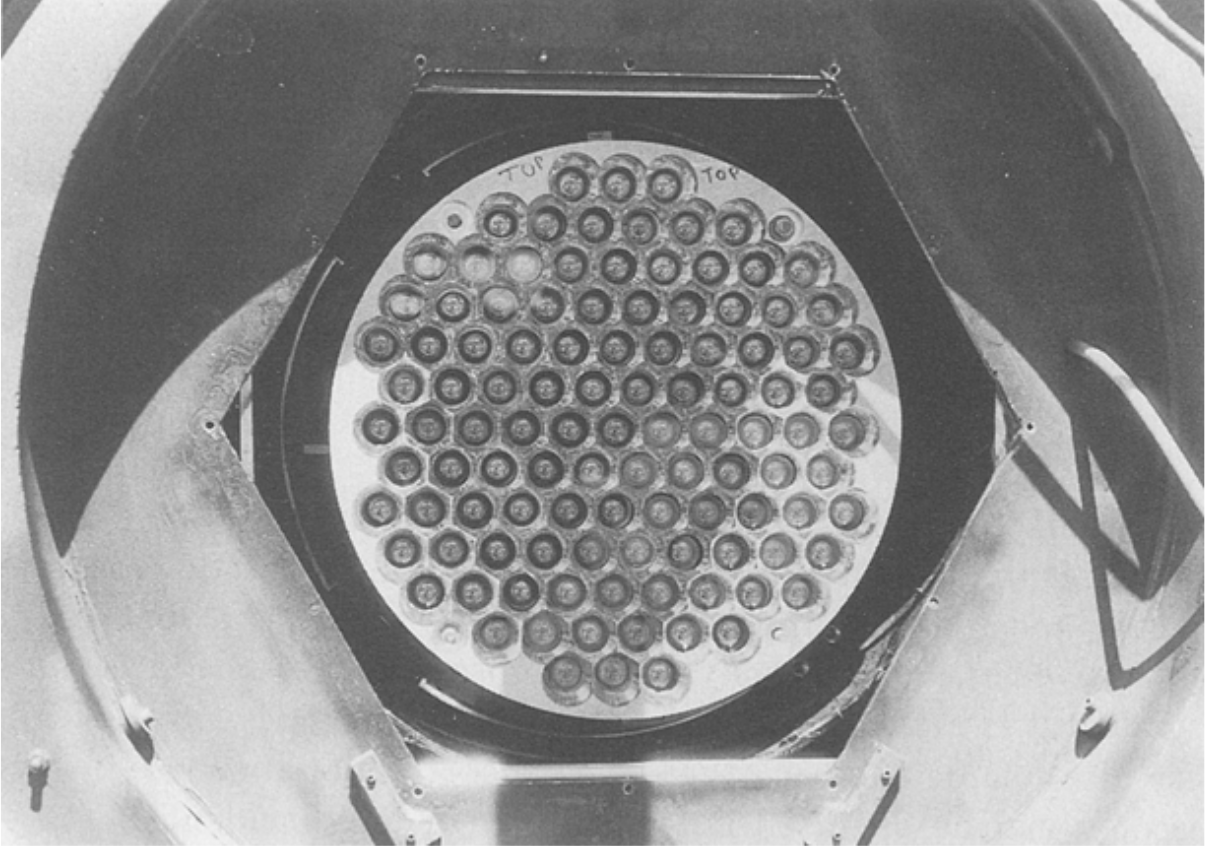
\includegraphics[width=0.8\textwidth]{images/whipple_cam.png}
    \caption{Picture of the upgraded camera of the Whipple telescope, installed in 1988 \cite{Cawley1995}.}  % not the best source
    \label{fig:whipple_cam}
\end{figure}

The shower images in combination with better computer simulations allowed for 
superior background rejection based on the  hillas-parameters.
1989 had the telescope observing the Crab Nebula with 9$\sigma$ 
\cite{1989ApJ...342..379W}.


Another big experiment of the time was the HEGRA experiment, an array consisting 
of 37 \SI{1}{\meter^2} scintillation detectors \cite{ALLKOFER1990345} in the first stage.
While at this stage not technically an IACT-experiment, later upgrade plans
brought multiple \SI{8.5}{\meter^2} diameter telescopes, starting with the first 
telescope in 1985 \cite{DAUM19971}.
While each telescope does not look too impressive on its own,
the so called HEGRA-IACT array made for a great use of the stereo principle,
marking the transition to the third generation of IACTs.


\subsection{The third generation}

Towards the end of the 1990s several third generation telescopes were
proposed:
H.E.S.S and MAGIC, deriving from parts of the HEGRA collaboration, 
VERITAS from Whipple and the no longer operating CANGAROO from Adelaide and 
several japanese universities \cite{HILLAS201319}.
All of these were designed as stereoscopic imaging telescopes building on the progress made during the 
second generation with two experiments located on each the north and the south hemisphere.

\subsubsection{Major Atmospheric Gamma Imaging Telescopes (MAGIC)}
MAGIC is a experiment initially operating as single telescope with a second slightly improved 
telescope added later \cite{BAIXERAS2003247}.
Both telescopes have a 17m diameter, 964 elements mirror.

- besonderheiten
- entdeckungen
- nutzung heute

\subsubsection{High Energy Stereoscopic System (H.E.S.S)}




\subsubsection{Very Energetic Radiation Imaging Telescope Array System (VERITAS)}



\section{Next to come: The Cherenkov Telescope Array (CTA)}


% bis vlt seite 15-25
